\documentclass{beamer}
\usepackage{caption}
\usetheme{Madrid}
\usecolortheme{beaver}
\usefonttheme{serif}
%\pgfdeclareimage[height=1.3cm]{logo}{fig/logo}
%\logo{\pgfuseimage{logo}}
\usepackage[framemethod=TikZ]{mdframed}
\usepackage{bookman} % the used font
\usepackage{booktabs} % Allows the use of \toprule, \midrule and \bottomrule in tables
\usepackage{amsmath,amsfonts,mathrsfs,amsthm,amssymb,ctex,tikz,bm,graphicx,hyperref,geometry,listings}
%\geometry{left=1cm,right=1cm}
\usepackage{gbt7714}
\definecolor{dkgreen}{rgb}{0,0.6,0}
\definecolor{gray}{rgb}{0.5,0.5,0.5}
\definecolor{mauve}{rgb}{0.58,0,0.82}
\lstset{
	frame=trbl,
	aboveskip=3mm,
	belowskip=3mm,
	showstringspaces=true,
	breaklines=true,
	columns=flexible,
	framerule=1pt,
	rulecolor=\color{gray},
	backgroundcolor=\color{white},
	basicstyle={\ttfamily},
	numbers=left,
	numbersep=1em,
	numberstyle=\color{black},
	keywordstyle=\color{blue},
	commentstyle=\color{gray},
	stringstyle=\color{mauve},
	tabsize=3,
}
\setbeamertemplate{caption}[numbered]
\setbeamersize{text margin left=10mm,text margin right=10mm}

\title[title]{Partial Differential Equations Theory}
\subtitle{答辩报告} % (optional)
\author[数学与统计学院]{李浩斌}

\institute[信阳师范大学]{信息与计算科学}
\date[\today] % (optional)
{\today}

%\AtBeginSection[]
%{
%	\begin{frame}
%		\frametitle{目录}
%		\everymath{\displaystyle}
%		\tableofcontents[currentsection]
%	\end{frame}
%}
\AtBeginEnvironment{theorem}{%
	\setbeamercolor{block title}{fg=white,bg=red!40}
	\setbeamercolor{block body}{fg=black,bg=gray!10}
}

\begin{document}
	\frame{\titlepage}
	
%	\begin{frame}
%	\frametitle{目录}
%		\tableofcontents
%	\end{frame}
	
\section{问题}
	\begin{frame}
		\frametitle{问题}
		\begin{itemize}
			\item \textbf{问题1:}
			\item \textbf{问题2:}
		\end{itemize}
	\end{frame}
	
\section{问题一}
	\begin{frame}
		\frametitle{问题一}
		这里输入文字
		\begin{columns}
			\begin{column}{0.5\textwidth}
				内容...
			\end{column}
			
			\begin{column}{0.5\textwidth}
				内容...
				\begin{figure}
					\centering
					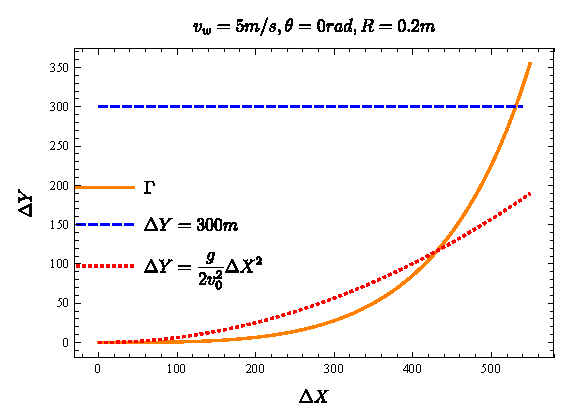
\includegraphics[width=\textwidth]{figure/hlx-q1}
					\caption{figure}
					\label{fig:hlx}
				\end{figure}
			\end{column}
		\end{columns}
	\end{frame}
	
	\begin{frame}{问题一}
		\begin{theorem}[PDE]
			here
		\end{theorem}
		\begin{definition}[additional text]
			内容...
		\end{definition}
	\end{frame}
	\begin{frame}
	\frametitle{问题二}
	以下是\texttt{matlab}代码
	\lstinputlisting[language=matlab]{code/matlab-code-q1.m} 
	

	\end{frame}

\section{标题2}
\begin{frame}
	\frametitle{第一部分}

\end{frame}

\begin{frame}
	\frametitle{第二部分}
	这里输入文字\cite{ref}
\end{frame}

\section{标题3}
\begin{frame}
	\frametitle{第一部分}
	这里输入文字
\end{frame}

\begin{frame}
	\frametitle{第二部分}
	这里输入文字
\end{frame}

\section{最后}
	\begin{frame}
		\frametitle{最后}
		\begin{figure}[H]
			\centering
			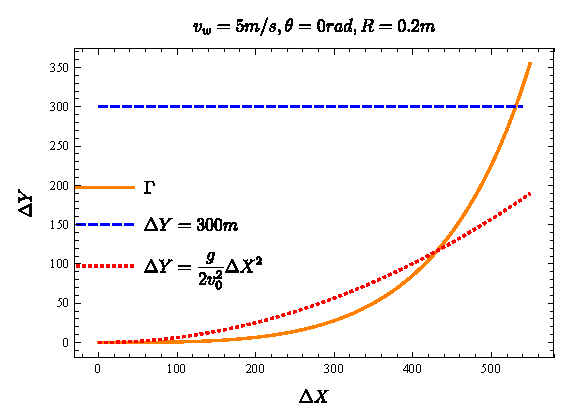
\includegraphics[width=0.6\linewidth]{figure/hlx-q1.eps}
			\caption{与理想状态下的对比图}
			\label{fig:hlx-q1}
		\end{figure}
	\end{frame}
	
	\begin{frame}
		\frametitle{第二部分}
	\end{frame}
	
\section{参考文献}
	\begin{frame}
		\frametitle{参考文献}
		\bibliography{ref/ref}
	\end{frame}
	\begin{frame}
		\Huge{\centerline{Thank you!}}
	\end{frame}
	
\end{document}